\section{联邦学习}

\subsection{联邦学习基本概念}
联邦学习(Federated Learning, FL)是一种分布式机器学习框架,在保障数据隐私的前提下,实现多方协同训练机器学习模型\cite{yang2019federated}。与传统集中式训练不同,联邦学习不要求上传原始数据到中央服务器,而是各参与方(客户端)在本地使用自身数据训练模型,仅上传模型更新(如参数梯度)至中央服务器进行聚合,从而形成全局模型,如图\ref{fig:federated_learning_workflow}所示。

\begin{figure}[htbp]
    \centering
    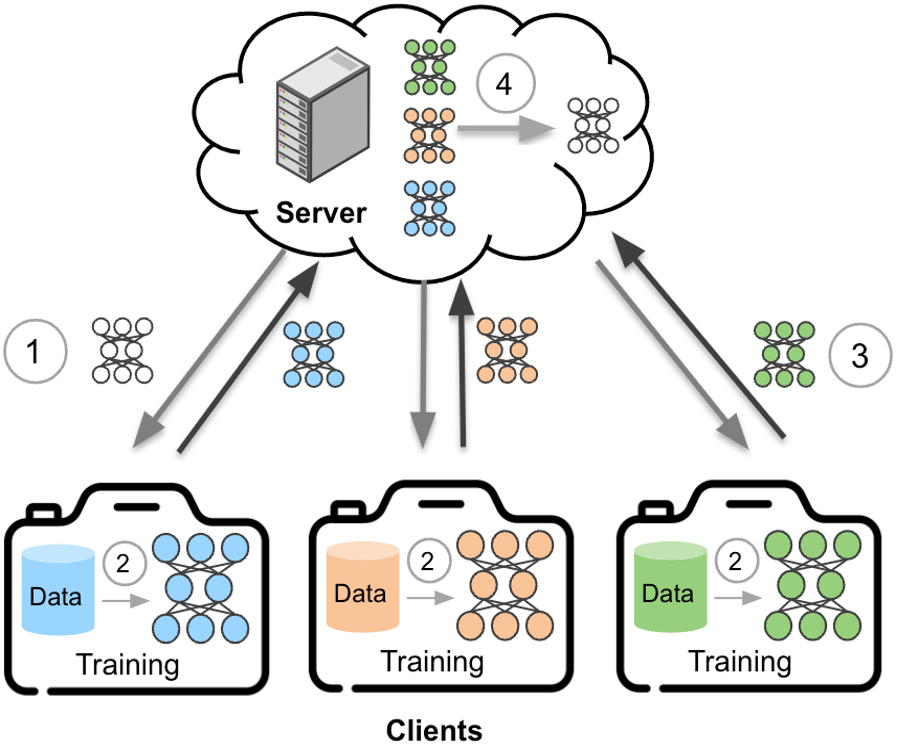
\includegraphics[width=0.6\textwidth]{Imgs/FL-structure.png}
    \caption{联邦学习工作流程总览图}
    \label{fig:federated_learning_workflow}
\end{figure}

该概念最早由Google于2016年提出\cite{mcmahan2017communication},其核心优势在于数据始终保留本地,避免了隐私泄露风险与法律合规问题,同时通过整合多方知识提升模型泛化性能。联邦学习已在医疗、金融、移动终端等数据敏感场景获得广泛应用\cite{zhang2024fedtgp, hard2018federated}。

\subsection{联邦学习的工作流程}
联邦学习的典型流程如图\ref{fig:fl_protocol_round}所示,主要包括以下步骤:

\begin{figure}[htbp]
    \centering
    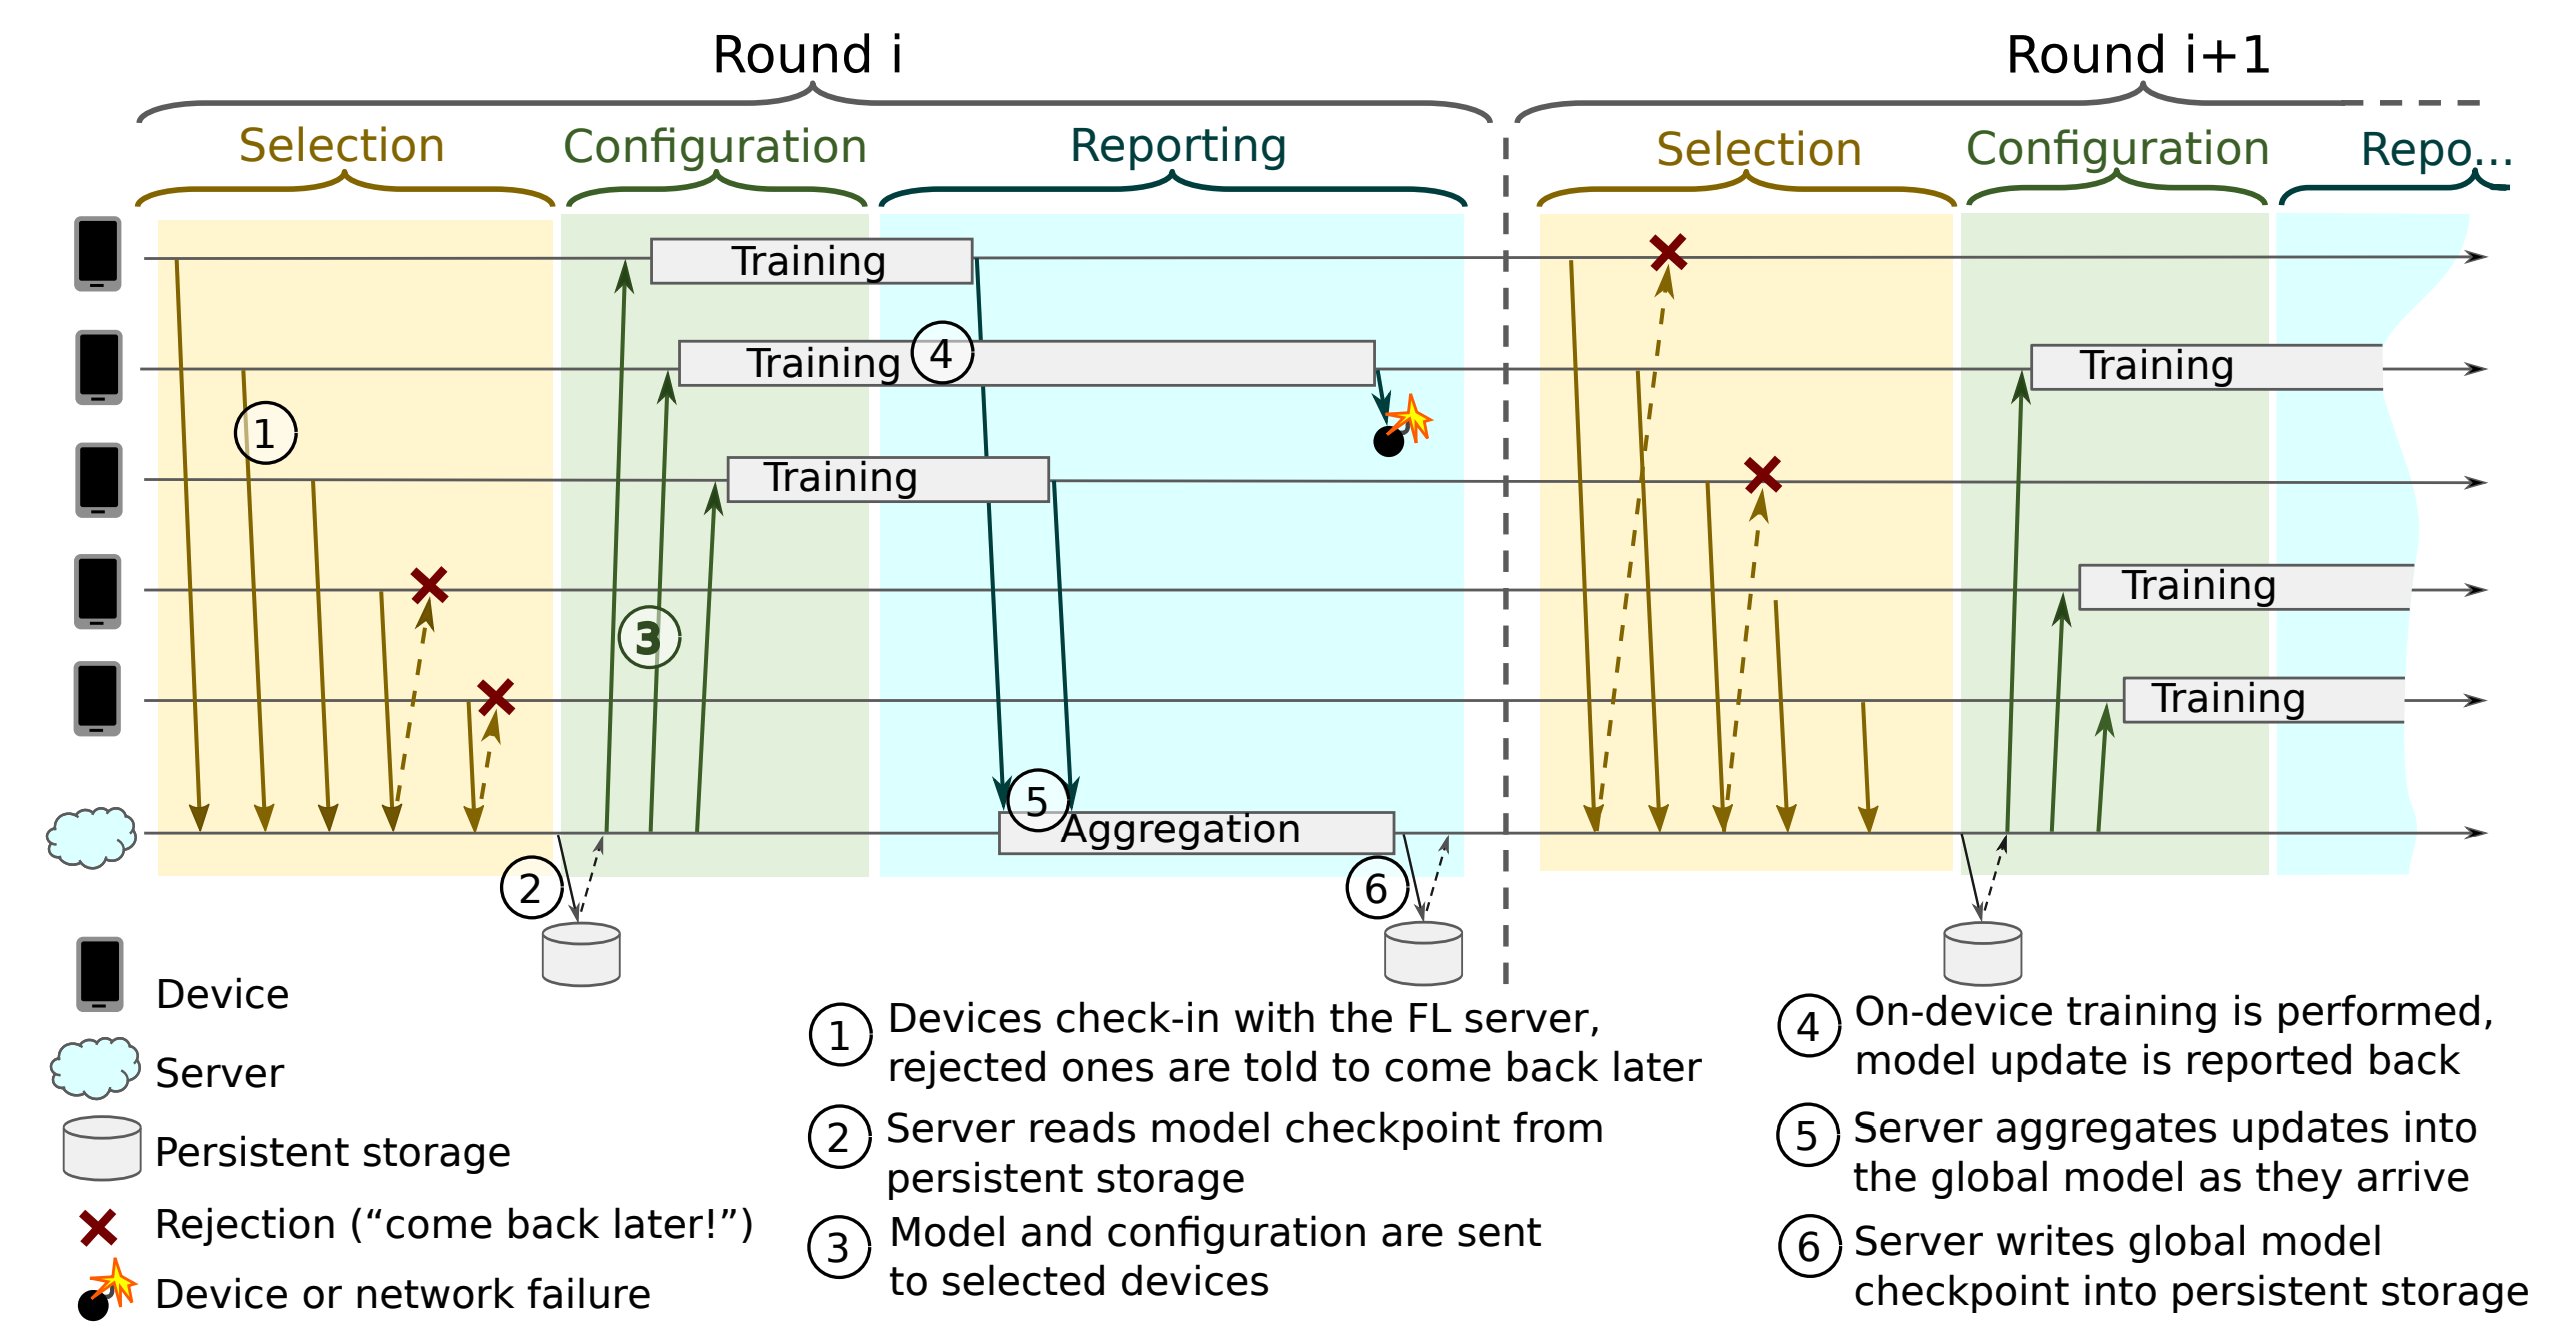
\includegraphics[width=\textwidth]{Imgs/FL-Learning-Protocol.png}
    \caption{典型联邦学习协议轮次流程示意图\cite{bonawitz2019towards}}
    \label{fig:fl_protocol_round}
\end{figure}

\begin{enumerate}[label=(\roman*)]% 注意标签label的使用
    \item \textbf{全局模型初始化与下发:} 服务器初始化全局模型并下发至客户端。
    \item \textbf{客户端本地训练:} 客户端在本地数据上进行模型训练,更新模型参数。
    \item \textbf{本地模型更新上传:} 客户端将加密后的模型更新(如梯度)上传至服务器。
    \item \textbf{全局模型聚合:} 服务器采用如FederatedAveraging等算法聚合客户端更新,形成新的全局模型。
    \item \textbf{循环迭代直至收敛:} 重复上述过程,直至模型收敛或达到设定轮次。
    \item \textbf{模型评估与部署:} 服务器对全局模型进行评估,若满足性能要求则部署至客户端。
\end{enumerate}

在整个过程中,原始数据从不离开本地,跨节点仅传递模型更新,可结合差分隐私、安全多方计算等技术进一步增强安全性与信任度。

\subsection{联邦学习的主要挑战}
尽管联邦学习在隐私保护方面具备优势,其分布式架构也带来了以下关键挑战\cite{zhu2023blockchain,li2020federated}:

\begin{itemize}
    \item \textbf{信任与安全挑战:} 依赖中心服务器存在单点故障与中毒攻击等安全隐患,需引入稳健聚合、差分隐私等机制提升安全性。
    \item \textbf{缺乏激励机制:} 缺乏合理激励可能导致参与方积极性不足或出现搭便车行为,影响整体训练质量。
    \item \textbf{统计异构性:} 各客户端数据分布差异显著(Non-IID问题),加剧模型收敛困难,影响全局模型泛化性。
    \item \textbf{系统异构性:} 设备性能与网络环境差异大,易产生“慢节点”问题,需设计容错与调度机制适应异构环境。
    \item \textbf{通信负担:} 多轮模型交换带来高通信开销与潜在窃听风险,需借助加密与通信压缩技术优化效率与安全。
    \item \textbf{法规约束:} 需遵循各国数据隐私法规(如GDPR)限制,设计合规的跨境协作方案\cite{li2019impact}。
\end{itemize}

综上,联邦学习在打破数据孤岛方面展现潜力,但仍需解决信任、激励与异构性等技术难题。为应对这些挑战,区块链的去中心化与可编程机制为联邦学习提供了重要补充。下一节将系统探讨区块链赋能下的数据共享机制设计。